\documentclass[12pt,a4paper,twoside]{report}

% -----------------------
% Encoding and language
% -----------------------
\usepackage[utf8]{inputenc}
\usepackage[T1]{fontenc}
\usepackage[english]{babel}

% -----------------------
% Spacing and layout
% -----------------------
\usepackage{setspace}
\setstretch{1.2}          % line spacing
\setlength{\parskip}{0.8em}
\setlength{\parindent}{0pt}

\usepackage[a4paper,top=2.5cm,bottom=2.5cm,left=2.5cm,right=2.5cm]{geometry}

% -----------------------
% Figures, floats, tables
% -----------------------
\usepackage{graphicx}
\usepackage{float}
\usepackage{subcaption}
\usepackage{array}
\usepackage{tabularx}
\usepackage{longtable}
\usepackage[table]{xcolor}
\usepackage{ragged2e}
\usepackage{placeins}   % for \FloatBarrier

\renewcommand{\arraystretch}{1.3} % increases row spacing in tables

% -----------------------
% Headers and footers
% -----------------------
\usepackage{fancyhdr}
\setlength{\headheight}{14.5pt}

\fancypagestyle{plain}{%
	\fancyhf{}%
	\renewcommand{\headrulewidth}{0pt}%
	\renewcommand{\footrulewidth}{0pt}%
}

\fancypagestyle{frontmatterstyle}{%
	\fancyhf{}%
	\fancyhead[LE,LO]{\nouppercase{\leftmark}}%
	\fancyhead[RE,RO]{2025--2024}%
	\renewcommand{\headrulewidth}{0.4pt}%
	\renewcommand{\footrulewidth}{0pt}%
}

\fancypagestyle{mainmatterstyle}{%
	\fancyhf{}%
	\fancyhead[LE,LO]{\nouppercase{\leftmark}}%
	\fancyhead[RE,RO]{2025--2024}%
	\fancyfoot[LE,LO]{Faculty of Science of Monastir (FSM)}%
	\fancyfoot[RO,RE]{\thepage}%
	\renewcommand{\headrulewidth}{0.4pt}%
	\renewcommand{\footrulewidth}{0.4pt}%
}	

% -----------------------
% Section title formatting
% -----------------------
\usepackage{titlesec}

\titlespacing*{\chapter}{0pt}{-1ex plus 0.5ex minus .2ex}{2ex plus .2ex}
\titlespacing*{\section}{0pt}{2ex plus 1ex minus .5ex}{1ex plus .5ex}
\titlespacing*{\subsection}{0pt}{2ex plus 1ex minus .5ex}{1ex plus .5ex}
\titlespacing*{\subsubsection}{0pt}{2ex plus 1ex minus .5ex}{1ex plus .5ex}

% -----------------------
% Lists
% -----------------------
\usepackage{enumitem}
\setlist{noitemsep, topsep=0pt}

% -----------------------
% Hyperlinks
% -----------------------
\usepackage{hyperref}
\hypersetup{
	colorlinks=true,
	linkcolor=blue,
	citecolor=blue,
	urlcolor=blue
}

% -----------------------
% Custom commands
% -----------------------
\definecolor{blue_}{RGB}{0,0,200}
\newcommand{\HRule}{\rule{\linewidth}{0.5mm}}





\begin{document}
	
	% ==== TITLE PAGE ====
	\begin{titlepage}
		\raggedright
		\noindent
		\begin{minipage}{0.2\textwidth}
			\includegraphics[scale=0.2]{images/logofsm.jpg}
		\end{minipage}%
		\begin{minipage}{0.6\textwidth}
			\centering
			\textsc{\large
				Republic of Tunisia \\
				University of Monastir \\
				Faculty of Sciences of Monastir \\
				Department of Computer Science}
		\end{minipage}%
		\begin{minipage}{0.2\textwidth}
			\raggedleft
			\includegraphics[height=2.5cm]{images/logouniv.jpg}
		\end{minipage}
		
		\vspace{1.5cm}
		\begin{center}
			{\large Thesis submitted for the degree of:}\\[0.3cm]
			{\Large \textbf{Professional Master in Data Science}}
		\end{center}
		
		\vspace{0.5cm}
		\HRule
		\begin{center}
			{\fontfamily{ptm}\selectfont \huge \bfseries \color{blue_}
				Intelligent Platform for Industrial Equipment, Document Management, and AI Support}
			
			\HRule \\[0.5cm]
			
			{\large Completed at: \textbf{LEONI}} \\[0.5cm]
			{\large Submitted by: \textbf{Chebaane Ismail}} \\[1cm]
			
			\begin{minipage}{0.45\textwidth}
				{\large Professional Supervisor:}\\
				\textbf{Mr. Nourddine Labiedh}
			\end{minipage}%
			\hfill
			\begin{minipage}{0.45\textwidth}
				{\large Academic Supervisor:}\\
				\textbf{Mr. Mouhamed Neji Maatouk}
			\end{minipage}\\[1.5cm]
			
			{\large Defended on \textbf{11/10/2025}, before:}\\[0.3cm]
			{\large President: \textbf{Mr.} \\ Reviewer: \textbf{Mr.}} \\[1cm]
			
			{\large Academic Year: 2025}\\
			{\large Location: Monastir, Tunisia}
		\end{center}
		
		\vfill
	\end{titlepage}
	
	\pagestyle{empty} % no numbering on dedication & acknowledgments
	
	% ==== DEDICATION ====
	\begin{center}
		{\Large \textbf{Dedication}}\\[1cm]
		\setstretch{1.15}
		\begin{itshape} \small To my dear father,\\[0.3cm] No words can truly capture the depth of my feelings for you.\\ It is thanks to your unwavering love, trust, patience, sacrifices,\\ and constant encouragement that I have reached this stage of my life.\\ I can only hope that I have been worthy of your affection and faith in me.\\[0.5cm] To my beloved mother,\\[0.3cm] You are my reason for being, my guiding light,\\ the gentle lantern that illuminates my path with love and warmth.\\ Words fall short when I try to express the immense gratitude, pride,\\ and deep love I hold for you.\\ For every sacrifice you have made for my success,\\ I pray that God grants you health, happiness, and a long, peaceful life.\\[0.5cm] To my siblings,\\[0.3cm] Thank you for your constant encouragement, your advice,\\ and your presence in my life.\\ I wish each of you a future filled with success, joy, and blessings,\\ and I pray that God keeps us forever united.\\[0.5cm] To my friends,\\[0.3cm] Your friendship has been a true gift.\\ Your respect, kindness, and readiness to help me at every step\\ will forever remain in my heart.\\ Together, we have overcome challenges and shared victories,\\ and for that I am eternally grateful.\\[0.5cm] To all those I love and who love me,\\[0.3cm] This work is dedicated to you.\\ It is my humble way of honoring the trust you placed in me\\ and fulfilling your wish to see me succeed. \end{itshape}
	\end{center}
	\clearpage
	
	% ==== ACKNOWLEDGMENTS ====
	\begin{center}
		{\Large \textbf{Acknowledgments}}\\[1.5cm]
		\setstretch{1.2}
		\begin{itshape} It is with great pleasure that I dedicate this page to express my sincere gratitude to all those who have made this study possible and contributed to its completion in various ways.\\[0.5cm] “Thank God for giving me the strength to accomplish my studies.”\\[1cm] I would like to sincerely thank my university supervisor, Mr. Mohamed Neji Maatouk, who honored me by guiding and reviewing this work. Your dedicated involvement through your insightful directives, remarks, suggestions, and encouragement during key moments has been invaluable. I am deeply grateful for your availability whenever I sought your support. Your dedication, wise advice, and kindness have truly made this journey enjoyable. Please accept my heartfelt thanks and highest appreciation.\\[1cm] My special thanks also go to my professional supervisors in the company, Mr. Nourddine Labiedh, Mr. Oussama Zegnani, and Ms. Jawher Zairi, whose generous help, precious advice, clear explanations, and constructive feedback greatly supported the realization of this project.\\[1cm] I am also very grateful to the members of the Jury for accepting, without reservation, to evaluate this work fairly and for their valuable remarks which, with time and reflection, will undoubtedly contribute to the improvement of this thesis. Your presence on the jury is a great honor to me, and I sincerely appreciate your commitment.\\[1cm] Finally, I would like to thank my institute for providing me with the opportunity to acquire such valuable training. \end{itshape}
	\end{center}
	\clearpage
	
	% ==== FRONTMATTER ====
	\pagenumbering{roman}
	\setcounter{page}{1}
	\pagestyle{frontmatterstyle}
	
	\tableofcontents
	\clearpage
	
	\listoftables
	\clearpage
	
	\listoffigures
	\clearpage
	
	% ==== MAINMATTER ====
	\pagenumbering{arabic}
	\pagestyle{mainmatterstyle}
	\raggedright
	
	\chapter*{General Introduction}
	\markboth{General Introduction}{}
	\addcontentsline{toc}{chapter}{General Introduction}
	
	In today’s industrial landscape, marked by rapid digital transformation, the competitiveness of companies increasingly depends on their ability to optimize equipment management and make effective use of data. Maintenance, document management, and equipment lifecycle monitoring have become strategic priorities, directly influencing productivity, efficiency, and long-term sustainability.
	
	However, many organizations still face challenges due to complex manual processes, limited access to information, and a lack of integrated tools for monitoring and anticipating failures. These constraints often result in time loss, administrative overload, and difficulties in making fast and informed decisions.
	
	To overcome these challenges, the integration of advanced technological solutions has become essential. Artificial Intelligence (AI), combined with process automation and document digitalization, offers promising opportunities. An intelligent chatbot capable of providing instant and contextualized assistance, together with a predictive model that estimates the remaining useful life of equipment, represents a valuable asset for reducing maintenance costs, increasing equipment availability, and enhancing decision-making.
	
	This dissertation focuses on the development of an intelligent web application that integrates several key components:
	\begin{itemize}
		\item an \textbf{AI-powered chatbot assistant} to support users in real time,
		\item a \textbf{prediction module} to estimate the remaining useful life of equipment,
		\item a \textbf{digitalization and electronic signature system} for technical documents,
		\item and a \textbf{centralized dashboard} for managing equipment and user data.
	\end{itemize}
	
	The ultimate goal of this project is to improve operational efficiency, facilitate data accessibility, and support decision-making processes within industrial environments.
	
	This work is structured into the following chapters:
	\begin{itemize}
		\item \textbf{Chapter 1: Project Context and Objectives} – This chapter introduces the project, its general framework, the identified problems, and the specific objectives. It also presents a critical analysis of existing systems.
		\item \textbf{Chapter 2: Needs Analysis and Design} – This section defines the actors and both functional and non-functional requirements, supported by various design models such as use case diagrams, class diagrams, and sequence diagrams.
		\item \textbf{Chapter 3: Implementation and Analysis of the Solution} – This chapter details the development of the intelligent chatbot, the predictive approaches adopted, as well as the final architecture of the system.
		\item \textbf{Chapter 4: Implementation and Evaluation} – The final chapter presents the working environment, the developed interfaces, and the evaluation of the obtained results.
	\end{itemize}
	
	\clearpage
	
	% =======================
	% Chapter 1 - Project Context and Objectives
	% =======================
	\chapter{Project Context and Objectives}
	
	\section{Introduction}
	
	In this chapter, we will first present the LEONI company along with its LTN3 site to provide the organizational and operational context of the project. Secondly, the context of the project and the problem statement will be examined to highlight the industrial challenges addressed. Then, the project objectives will be defined, clarifying the goals we aim to achieve. Following this, a study of existing systems on the market will be conducted, including an analysis and critique of their strengths and weaknesses. Finally, the chapter will conclude by introducing the proposed solution developed to overcome the identified limitations and meet the project objectives.
	
	
	
	\section{Presentation of LEONI Company and the LTN3 Site}
	
	\subsection{LEONI Tunisia}
	
	\subsubsection*{a) Organization of LTN}
	
	The organizational chart of \textbf{LEONI Tunisia} is shown in Figure~\ref{fig:organigramme_leoni}.
	
	\begin{figure}[H]
		\centering
		\includegraphics[width=0.9\textwidth]{figures/organigramme_leoni.jpg}
		\caption{Organizational chart of LEONI Tunisia}
		\label{fig:organigramme_leoni}
	\end{figure}
	
	\subsubsection*{b) LEONI Sites in Tunisia}
	
	Since 1977, LEONI Tunisia has continuously grown. It currently has five production sites illustrated in Figure~\ref{fig:sites_leoni}: Menzel Hayet, Mateur South, Mateur North, Sidi Bouali, and Sousse.
	
	\begin{figure}[H]
		\centering
		\includegraphics[width=0.9\textwidth]{figures/sites_leoni.jpg}
		\caption{LEONI Sites in Tunisia}
		\label{fig:sites_leoni}
	\end{figure}
	
	\subsubsection*{c) LEONI Clients}
	
	The main clients of LEONI are:
	
	\begin{itemize}
		\item MERCEDES BENZ
		\item Volkswagen
		\item AUDI
		\item BMW
		\item Peugeot
		\item Citroën
		\item FIAT
		\item PORSCHE
		\item BENTLEY
		\item etc.
	\end{itemize}
	
	\begin{figure}[H]
		\centering
		\includegraphics[width=0.9\textwidth]{figures/clients_leoni.jpg}
		\caption{Clients of LEONI}
		\label{fig:clients_leoni}
	\end{figure}
	
	\subsubsection*{d) LEONI Suppliers}
	
	LEONI’s suppliers are:
	
	\begin{itemize}
		\item \textbf{International:} Siemens, Delphi, Power-Pecker, Continental.
		\item \textbf{National:} A.A.F. Electronics, Coficab, Tyco Electronics AMP GmbH, LEONI Roth, Hellermann Tyton GmbH, Delphi Automotive Systems, Fuba Automotive GmbH.
	\end{itemize}
	
	\subsubsection*{e) LEONI Tunisia Certifications and Awards}
	
	LEONI Tunisia is recognized as a leader in automotive wiring. Its international certifications testify to its commitment to quality and environment. The certifications obtained are:
	
	\begin{itemize}
		\item ISO/TS 16949 version 2009
		\item ISO 9001 version 2015
		\item ISO 14001 version 2004
	\end{itemize}
	
	Additionally, LEONI has received several qualification awards from various departments (Figure~\ref{fig:prix_leoni}).
	
	\begin{figure}[H]
		\centering
		\includegraphics[width=0.9\textwidth]{figures/prix_leoni.jpg}
		\caption{Qualification awards of LEONI Tunisia}
		\label{fig:prix_leoni}
	\end{figure}
	
	\subsubsection*{f) Main Competitors}
	
	In a highly competitive market, LEONI strives to satisfy and retain clients to strengthen its market position. The main competitors in the automotive wiring sector are presented in Figure~\ref{fig:concurrents_leoni}.
	
	\begin{figure}[H]
		\centering
		\includegraphics[width=0.9\textwidth]{figures/concurrents_leoni.jpg}
		\caption{Main competitors of LEONI}
		\label{fig:concurrents_leoni}
	\end{figure}
	
	\subsection*{1.2.2 LEONI Messadine LTN3}
	
	The internship took place at LTN 3, the third expansion established in 2004. This site includes four buildings classified by client (Figure~\ref{fig:ltn3_batiments}):
	
	\begin{itemize}
		\item LTN 3 A: OEM Germany (various clients from Germany and the UK)
		\item LTN 3 B: OEM France (clients BOSCH and SCANIA)
		\item LTN 3 C: Mercedes Benz client
		\item LTN 3 D: BMW client
	\end{itemize}
	
	\begin{figure}[H]
		\centering
		\includegraphics[width=0.9\textwidth]{figures/ltn3_batiments.jpg}
		\caption{LEONI Messadine LTN3}
		\label{fig:ltn3_batiments}
	\end{figure}
	
	\subsubsection*{a) Presentation of LTN3}
	
	The production unit "OEM SUPPLIER GR" LEONI Tunisia follows a policy of expanding its activity domain to win new markets and improve international competitiveness. The OEM SUPPLIER GERMANY project was launched in Sousse in 2007 at LTN 3 (LEONI Tunisia 3).
	
	\paragraph{Organizational Chart of LTN3}
	
	The LEONI site "OEM SUPPLIER GR" plant section is a divisionally structured company. It has 8 departments cooperating to achieve common objectives (Figure~\ref{fig:organigramme_ltn3}).
	
	\begin{figure}[H]
		\centering
		\includegraphics[width=0.9\textwidth]{figures/organigramme_ltn3.jpg}
		\caption{Organizational chart of LTN3}
		\label{fig:organigramme_ltn3}
	\end{figure}
	
	The organizational chart shows different cooperating departments, summarized below:
	
	\begin{itemize}
		\item \textbf{OPEX Department:} Minimize non-value-added tasks through continuous improvement and interdepartmental communication.
		\item \textbf{Production Department:} Ensure smooth production according to scheduling.
		\item \textbf{Quality Department:} Minimize defects to satisfy the client.
		\item \textbf{Logistics Department:} Plan manufacturing orders and manage the supply chain.
		\item \textbf{Engineering Department:} Composed of three services:
		\begin{itemize}
			\item Ratio Service (IE): Methods and work rules.
			\item Study Service (SE): Analysis of assembly drawings.
			\item Development Service (AV): New product studies.
		\end{itemize}
		\item \textbf{Finance Department:} Prepares financial statements, analyzes profitability, and participates in strategic decisions.
		\item \textbf{Technical Department:} Corrective/preventive maintenance, equipment control and installation.
		\item \textbf{Human Resources Department (HR):} Personnel management, recruitment, and working conditions.
	\end{itemize}
	
	\paragraph{Layout of LTN3: Plant Section OEM SUPPLIER GR}
	
	The plant is divided into 8 sections (Figure~\ref{fig:layout_ltn3}):
	
	\begin{itemize}
		\item Import warehouse: storage of raw materials (coils, containers).
		\item SEG cutting: automatic wire cutting and crimping.
		\item SEG VKF: pre-assembly, wire preparation, and storage (Pagoda).
		\item SEG 42: cable assembly for clients Continental and Vitesco.
		\item SEG UK: cable assembly for clients Varroc, ZKW, Marelli.
		\item SEG 47: cable assembly for clients Cockpit, ZF, MEKRA.
		\item SEG 44: cable assembly for clients Brose, Isri, Inalfa, Magna, Seat Ateca, ZKW SCALA.
		\item Export warehouse: storage of finished products.
	\end{itemize}
	
	\begin{figure}[H]
		\centering
		\includegraphics[width=0.9\textwidth]{figures/layout_ltn3.jpg}
		\caption{LAY-OUT OEM SUPPLIER GERMANY}
		\label{fig:layout_ltn3}
	\end{figure}
	
	\subsection*{1.2.3 Hosting Department: Capacity Planning, Capex and Fixed Assets}
	
	The internship was carried out in the Capacity Planning \& Capex and Fixed Assets department. This department plays a strategic role in managing material resources and industrial planning in the medium and long term.
	
	Its main mission is to anticipate, plan, and adjust production capacities according to demand forecasts, while managing investments and fixed assets.
	
	The department is responsible for:
	
	\begin{itemize}
		\item Developing capacity plans in coordination with production, logistics, and engineering.
		\item Managing investment requests (Capex) from need to budget approval.
		\item Tracking fixed assets: registration, allocation, transfers, decommissioning.
		\item Optimizing material resource usage.
		\item Providing regular reporting to management.
	\end{itemize}
	
	It acts as an interface between finance, production, maintenance, and industrial management.
	
	\subsection*{1.2.4 Presentation of the Production Process}
	
	\subsubsection*{1.2.4.1 Import Warehouse}
	
	Place for storing raw materials upon reception (joints, rolls, clips, wires, etc.).
	
	\subsubsection*{1.2.4.2 Cutting}
	
	First value-added step performed by automated machines:
	
	\begin{itemize}
		\item Cutting cables to specified lengths.
		\item Partial stripping of wires.
		\item Crimping contacts at ends.
		\item Twisting according to requirements.
	\end{itemize}
	
	\subsubsection*{1.2.4.3 PAGODA before VKF}
	
	Storage warehouse for lots of cut wires:
	
	\begin{itemize}
		\item Lot grouping.
		\item Barcode registration.
		\item FIFO storage.
	\end{itemize}
	
	\subsubsection*{1.2.4.4 Pre-assembly}
	
	Preparation of essential sub-assemblies considered as semi-finished products.
	
	\subsubsection*{1.2.4.5 Assembly}
	
	Final assembly of wires and sub-assemblies according to technical boards:
	
	\begin{itemize}
		\item Linked workstations (LAD): series production of simple products.
		\item Conventional chains (LAC): assembly of complex wiring.
		\item Carousels: medium complexity wiring, convertible to LAD double output.
		\item Fixed stations (PF): independent, for optional products or X-code /  Pro-Vermontage.
	\end{itemize}
	
	\section{Context of the Project}
	
	This project was carried out as part of an end-of-studies internship at \textbf{LEONI Wiring Systems}, a multinational company specialized in manufacturing automotive wiring harnesses. It was initiated to address the growing industrial need for a modern, intelligent, and user-friendly digital platform.  
	
	The solution aims to centralize equipment management, digitize technical documentation, and integrate an AI-powered chatbot for instant, context-aware assistance. It also includes a predictive model to estimate the Remaining Useful Life (RUL) of equipment, enabling proactive and optimized maintenance planning. The work was developed in close collaboration with the maintenance, production, and IT departments to ensure that it meets real operational requirements and improves overall efficiency.
	
	\section{Problem Statement}
	
	In many industrial environments, equipment management and technical documentation are handled through fragmented systems or manual processes. This often results in difficulties accessing critical information, delays in decision-making, and inefficiencies in maintenance planning.  
	
	At LEONI Wiring Systems, these challenges are further amplified by the need to maintain a large fleet of equipment while ensuring minimal downtime and strict compliance with production schedules. The absence of a unified platform integrating equipment tracking, document digitization, and predictive maintenance tools leads to operational gaps and increased maintenance costs.  
	
	
	\section{Project Objectives}
	
	The primary objective of this project is to design and develop an intelligent web application that addresses the identified industrial challenges. Specifically, the platform aims to:  
	
	\begin{itemize}
		\item Centralize equipment data and technical documentation in a unified digital environment.
		\item Integrate an AI-powered chatbot for instant and accurate assistance related to equipment and maintenance procedures.
		\item Implement a predictive model to estimate the Remaining Useful Life (RUL) of equipment, enabling proactive maintenance planning.
		\item Enhance operational efficiency, reduce downtime, and support data-driven decision-making.  
	\end{itemize}
	
	
	
	
	
	
	
	
	\section{Existing System Study}
	
	Understanding the current landscape of industrial equipment management and AI-assisted maintenance tools is essential for positioning our project effectively. This study reviews the main competitive systems and platforms available in the market, both commercial and open-source, focusing on their capabilities, strengths, and weaknesses.
	
	
	
	\section{Analysis of the Existing Systems}
	
	% Example with minipages to place image and text side by side
	\begin{minipage}{0.3\textwidth}
		\includegraphics[width=\linewidth]{figures/ibm_maximo_logo.svg} % your image path here
	\end{minipage}
	\hfill
	\begin{minipage}{0.65\textwidth}
		\textbf{IBM Maximo:} A leading Enterprise Asset Management (EAM) software, offering comprehensive equipment tracking, maintenance scheduling, and analytics. It supports AI integration but often requires substantial customization and investment.
	\end{minipage}
	
	\vspace{1em}
	
	\begin{minipage}{0.3\textwidth}
		\includegraphics[width=\linewidth]{figures/sap_eam_logo.jpg}
	\end{minipage}
	\hfill
	\begin{minipage}{0.65\textwidth}
		\textbf{SAP EAM:} Another major EAM platform integrating with SAP ERP systems, providing asset lifecycle management and predictive maintenance modules. Its complexity and cost can be barriers for medium-sized sites.
	\end{minipage}
	
	\vspace{1em}
	
	\begin{minipage}{0.3\textwidth}
		\includegraphics[width=\linewidth]{figures/microsoft_dynamics_logo.png}
	\end{minipage}
	\hfill
	\begin{minipage}{0.65\textwidth}
		\textbf{Microsoft Dynamics 365 Field Service:} Offers resource scheduling, asset management, and IoT integration, along with AI-powered virtual assistants. It is flexible but may require additional configuration for specific industrial domains.
	\end{minipage}
	
	\vspace{1em}
	
	\begin{minipage}{0.3\textwidth}
		\includegraphics[width=\linewidth]{figures/zendesk_logo.png}
	\end{minipage}
	\hfill
	\begin{minipage}{0.65\textwidth}
		\textbf{Zendesk and Intercom:} Widely used customer support chatbot platforms that provide automated responses, knowledge base integration, and user engagement tools. While powerful for customer service, they are not tailored for industrial equipment management.
	\end{minipage}
	
	\vspace{1em}
	
	\section{Critique of the Existing Systems}
	
	\begin{table}[H]
		\centering
		\resizebox{\textwidth}{!}{%
			\begin{tabular}{|l|c|c|c|}
				\hline
				\textbf{Criteria} & \textbf{Zendesk} & \textbf{Intercom} & \textbf{IBM Maximo Chatbot Module} \\
				\hline
				Customization & Limited & Advanced & Moderate \\
				\hline
				Natural Language Understanding & Limited & Good but sometimes inaccurate & Moderate \\
				\hline
				Cost & High & High & Very High \\
				\hline
				Ease of Deployment & Moderate & Easy & Complex \\
				\hline
				Industry Adaptability & Generic & Generic & Industry-specific \\
				\hline
				Resource Consumption & Low & Low & High \\
				\hline
				Response Speed & Fast & Fast & Moderate \\
				\hline
				Need for Model Retraining & High & High & High \\
				\hline
				Visual/Diagram Generation & No & No & Limited \\
				\hline
				Multilingual Support & Basic & Basic & Moderate \\
				\hline
			\end{tabular}%
		}
		\caption{Comparison of Existing Chatbot Solutions}
		\label{tab:chatbot_comparison}
	\end{table}
	
	Key limitations identified in current systems include:
	
	\begin{itemize}
		\item \textbf{High Cost and Resource Usage:} Enterprise platforms like IBM Maximo and SAP EAM require significant investments in licenses, hardware, and dedicated IT staff.
		\item \textbf{Lack of Industry-Specific AI Assistance:} Generic chatbots such as Zendesk and Intercom offer broad functionality but do not provide domain-specific expertise or predictive maintenance capabilities critical for industrial environments.
		\item \textbf{Limited Visual Interaction:} Most existing chatbots do not generate dynamic visual content such as charts or diagrams, restricting their ability to communicate complex data insights effectively.
		\item \textbf{Basic Multilingual Support:} Many solutions support only limited languages or lack robust multilingual natural language understanding, impacting accessibility in global industrial contexts.
		\item \textbf{Complex Deployment and Maintenance:} Many existing solutions demand complex setup processes and continuous model retraining or fine-tuning whenever new data or knowledge is added.
		\item \textbf{Fragmented Systems:} Current tools often specialize in either equipment management or AI assistance, rarely delivering both in an integrated, lightweight platform.
	\end{itemize}
	
	\section{Proposed Solution}
	
	Our project introduces an integrated, intelligent web application specifically designed for industrial equipment management, technical document digitization, and AI-driven user support.
	
	Key features and benefits include:
	
	\begin{itemize}
		\item \textbf{AI Chatbot with Dynamic Adaptability:} The chatbot leverages an advanced language model hosted online, providing fast and accurate responses without relying on local computing resources. Crucially, it can dynamically adapt to updated or new data without requiring retraining or fine-tuning, ensuring seamless integration of new information and continuous improvement.
		\item \textbf{Visual and Multilingual Capabilities:} Unlike many existing systems, our chatbot can generate dynamic visual outputs such as charts and diagrams to better illustrate data insights. It also supports advanced multilingual natural language understanding, making it accessible to diverse users in industrial environments.
		\item \textbf{High-Accuracy Prediction Model:} A dedicated module estimates the Remaining Useful Life (RUL) of equipment with approximately 89\% accuracy, enabling proactive and efficient maintenance scheduling.
		\item \textbf{Lightweight and Scalable Architecture:} The AI system is hosted on cloud servers rather than on local hardware, which eliminates the need for expensive or powerful equipment on-site. This approach allows the platform to easily support many users at once without performance issues. As a result, the solution is both cost-effective and scalable, able to grow and handle increased demand as needed.
		\item \textbf{Centralized Data Management:} The platform consolidates equipment details and maintenance histories into a single system to improve data accessibility and support informed decision-making.
		\item \textbf{User-Friendly Design:} Intuitive interfaces tailored for operators and engineers minimize training time and promote widespread adoption.
	\end{itemize}
	
	This solution addresses the limitations of existing platforms by combining advanced AI capabilities with industry-specific functionality, cost efficiency, and simplified deployment and maintenance.
	
	\section*{Conclusion}
	
	
	
	This chapter has provided a comprehensive overview of the project context by introducing the LEONI company and the LTN3 site where the internship took place. We have outlined the key industrial challenges motivating the project and defined clear objectives to address these issues. The study and critique of existing systems have highlighted the gaps and limitations in current solutions. Finally, the chapter introduced the proposed intelligent web application designed to integrate equipment management, digital documentation, and AI-assisted maintenance, setting the stage for the detailed development and implementation described in the following chapters.
	
	
	
	
	
	
	
	
	\chapter{Needs Analysis and Design}
	
	\section{Introduction}
	
	
	This chapter focuses on the needs analysis and design of the platform. It identifies the main actors—users, administrators, and the AI Chatbot—and their roles and interactions. Functional and non-functional requirements are detailed to ensure the system meets performance, usability, and security standards. The chapter also presents workflows, UML diagrams (use case, class, and sequence), and a data dictionary to clearly define system behavior, structure, and data attributes. This analysis provides a solid foundation for system implementation.
	
	\section{Identification of Actors}
	
	The system involves three main actors:
	
	\begin{itemize}
		\item \textbf{User:}  
		The end-user can:
		\begin{itemize}
			\item Navigate and search for equipment information.
			\item View dashboards displaying relevant metrics and statistics.
			\item Download or sign documents.
			\item Access the prediction module to estimate equipment Remaining Useful Life (RUL).
			\item Interact with the chatbot for equipment-related inquiries.
		\end{itemize}
		
		\item \textbf{Admin:}  
		The administrator has all the user capabilities plus additional management features:
		\begin{itemize}
			\item Manage user accounts (add, remove, update).
			\item Manage equipment records (add, remove, update).
			\item Upload, associate, and manage documents linked to equipment.
			\item Access notifications when users have more than 10 unsigned documents.
			\item Use the prediction module and chatbot.
		\end{itemize}
		
		\item \textbf{AI Chatbot:}  
		An intelligent assistant integrated into the platform that:
		\begin{itemize}
			\item Answers questions using a CSV database containing equipment information.
			\item Supports multiple languages for diverse user needs.
			\item Can generate and return diagrams when relevant.
		\end{itemize}
	\end{itemize}
	
	\section{Identification of Requirements}
	
	\subsection{Functional Requirements}
	
	The functional requirements of the system are as follows:
	
	\begin{itemize}
		\item \textbf{Equipment Management:} Ability to add, update, delete, and view equipment data.
		\item \textbf{Document Management:} Upload, view, sign, and track documents linked to equipment.
		\item \textbf{User Management (Admin only):} Create, update, and remove user accounts.
		\item \textbf{Dashboard Visualization:} Display statistics, KPIs, and monitoring charts.
		\item \textbf{Prediction Module:} Estimate the Remaining Useful Life (RUL) of equipment.
		\item \textbf{Notifications:} Alert admin when users have more than 10 unsigned documents.
		\item \textbf{Chatbot Interaction:} Provide answers, multilingual support, and diagrams from CSV data.
	\end{itemize}
	
	
	
	
	
	
	\subsection{Non-Functional Requirements}
	
	The non-functional requirements include:
	
	\begin{itemize}
		\item \textbf{Performance:} The system should respond to user actions in less than 2 seconds on average.
		\item \textbf{Scalability:} Support simultaneous access by multiple users without performance degradation.
		\item \textbf{Security:} Ensure secure authentication and protect sensitive data.
		\item \textbf{Usability:} Provide an intuitive and user-friendly interface for both users and admins.
		
		\item \textbf{Compatibility:} Accessible via major web browsers and mobile devices.
		\item \textbf{Multilingual Support:} The chatbot and UI must handle multiple languages seamlessly.
	\end{itemize}
	
	
	
	
	
	
	
	\section{Chatbot Operation Workflow}
	
	The chatbot is a key feature of the platform, enabling intelligent, multilingual interaction with users. Its operation is structured as follows:
	
	\begin{enumerate}
		\item \textbf{Data Loading:}  
		The chatbot uses a CSV file (\texttt{latest\_dataset.csv}) containing updated equipment data. This file is loaded into a Pandas \texttt{DataFrame} when the application starts.
		
		\item \textbf{Request Handling:}  
		When a user submits a question via the interface, it is sent as a JSON request to the Flask backend through the \texttt{/chat} API endpoint.
		
		\item \textbf{Custom Prompt Generation:}  
		The backend creates a structured prompt containing:
		\begin{itemize}
			\item The user’s question.
			\item The DataFrame columns.
			\item Instructions to return Python code for analysis or visualization only.
		\end{itemize}
		
		\item \textbf{Language Model Processing:}  
		The prompt is processed by a large language model through the Groq API. The model generates code to answer the query or create diagrams.
		
		\item \textbf{Execution and Diagram Generation:}  
		Using the PandasAI \texttt{SmartDataframe}, the generated code is executed. If a chart is created, it is saved in the \texttt{exports/charts} directory.
		
		\item \textbf{Response Delivery:}  
		\begin{itemize}
			\item Text results are returned directly to the user.
			\item Image results return a URL to the generated diagram.
		\end{itemize}
		
		\item \textbf{Multilingual Support:}  
		The model supports multiple languages, allowing users to interact in their preferred language without retraining the chatbot.
	\end{enumerate}
	
	This design allows the chatbot to adapt dynamically to updated CSV data without the need for retraining, ensuring continuous relevance and accuracy.
	
	
	
	
	
	\section{Use Case Diagrams}
	
	UML use case diagrams describe the main functionalities of the system and show the interactions between the system and its actors. 
	They provide a simple and clear way to visualize the possible actions for each actor.
	
	\subsection{Global Use Case Diagram}
	
	The global use case diagram presents an overview of the interactions between all actors and the system. 
	It highlights the different use cases that meet the defined functional requirements.
	
	\begin{figure}[H]
		\centering
		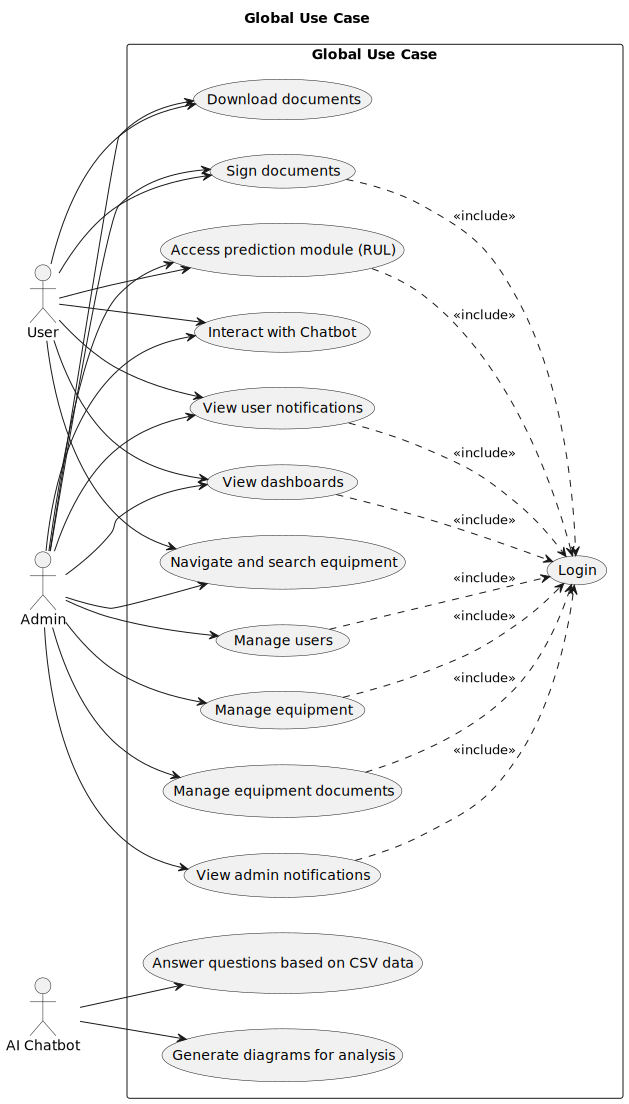
\includegraphics[width=\textwidth,height=0.9\textheight,keepaspectratio]{figures/use_case_global.pdf}
		\caption{Global Use Case Diagram}
		\label{fig:use_case_global}
	\end{figure}
	
	\subsection{Detailed Use Case Diagram – User}
	
	The detailed use case diagram for the User actor presents the specific interactions that a User can perform within the system. 
	It includes functionalities such as navigating equipment, viewing dashboards, using the prediction module, and interacting with the chatbot.
	
	\begin{figure}[H]
		\centering
		\includegraphics[width=\textwidth,height=0.8\textheight,keepaspectratio]{figures/use_case_user.pdf}
		\caption{Detailed Use Case Diagram – User}
		\label{fig:use_case_user}
	\end{figure}
	
	
	
	
	
	\begin{longtable}{|p{3cm}|p{10cm}|}
		\caption{Detailed Use Case Description — Interact with Chatbot} \\
		
		\hline
		\textbf{Title} & Interact with Chatbot \\ \hline
		\textbf{Description} & This use case allows the user to ask questions about equipment and generate diagrams for analysis. The system interprets the query and returns either textual answers or charts. \\ \hline
		\textbf{Actor} & User \\ \hline
		\textbf{Precondition} & The system has access to the latest equipment data in CSV format. The chatbot service is running and accessible. \\ \hline
		\textbf{Trigger} & The user opens the chatbot interface and submits a question. \\ \hline
		\textbf{Main Scenario} & 
		\begin{enumerate}
			\item User enters a question in the chatbot interface.
			\item System processes the query and generates the response.
			\item System returns either text or a diagram/chart.
			\item User views the response.
		\end{enumerate} \\ \hline
		\textbf{Alternative Scenario} &
		\begin{itemize}
			\item CSV file is outdated or missing: system shows an error.
			\item Diagram generation fails: system returns only textual response.
		\end{itemize} \\ \hline
		\textbf{Postconditions} & User receives an answer or a chart representing the requested analysis. \\ \hline
		\textbf{Benefits} & Enables users to get quick insights from equipment data and generate visual analysis without manual processing. \\ \hline
		
	\end{longtable}
	
	
	% End of previous section
	\clearpage % ensures tables/figures don’t overlap with new section
	
	\section{Class Diagram}
	
	The class diagram illustrates the main classes in the system, their attributes, methods, and the relationships between them. It provides a static view of the system structure, showing how objects interact and depend on each other.
	
	\begin{figure}[H]
		\centering
		\includegraphics[width=\textwidth,height=0.9\textheight,keepaspectratio]{figures/class_diagram.pdf}
		\caption{Class Diagram of the System}
		\label{fig:class_diagram}
	\end{figure}
	
	
	\section{Dictionnaire des Données}
	
	The data dictionary provides a detailed description of each attribute in the system's database. It includes the data type, the role of each attribute, and any constraints. This guide is essential for developers and system designers to understand the database structure and operation.
	
	\subsection{User}
	\vspace{-0.5cm} % reduce vertical space
	\begin{table}[H]
		\centering
		\begin{tabular}{|p{4cm}|p{3cm}|p{8cm}|}
			\hline
			\textbf{Attribute} & \textbf{Type} & \textbf{Description} \\ \hline
			id & String & Unique identifier of the user (primary key) \\ \hline
			fullName & String & Full name of the user \\ \hline
			username & String & Username for authentication \\ \hline
			matricule & String & Employee or system matricule number \\ \hline
			work & Enum (Work) & User's work type (QM, PPE, IM, SHEE) \\ \hline
			role & Enum (Role) & Role of the user (ADMIN, USER) \\ \hline
			notifications & List<Notification> & List of notifications received by the user \\ \hline
		\end{tabular}
		\caption{Data Dictionary for User}
	\end{table}
	
	\subsection{Equipment}
	\vspace{-0.5cm} % reduce vertical space
	\begin{table}[H]
		\centering
		\begin{tabular}{|p{4cm}|p{3cm}|p{8cm}|}
			\hline
			\textbf{Attribute} & \textbf{Type} & \textbf{Description} \\ \hline
			id & String & Unique identifier of the equipment (primary key) \\ \hline
			plant & Enum (PlantType) & Type of plant (MS, MN, etc.) \\ \hline
			equipmentName & String & Name of the equipment \\ \hline
			technicalId & String & Technical identifier \\ \hline
			process & String & Manufacturing or production process \\ \hline
			masterDataName & String & Master data reference name \\ \hline
			location & Enum (LocationType) & Location of equipment within the plant \\ \hline
			serialNumber & String & Equipment serial number \\ \hline
			year & Integer & Year of production \\ \hline
			equipmentStatus & String & Current status (e.g., Validated, Pending) \\ \hline
			Rul & Integer & Remaining Useful Life of the equipment \\ \hline
			documents & List<DocumentEntity> & List of documents related to the equipment \\ \hline
			archive & List<DocumentEntity> & Archived documents \\ \hline
		\end{tabular}
		\caption{Data Dictionary for Equipment}
	\end{table}
	
	\subsection{DocumentEntity}
	\begin{table}[H]
		\centering
		\begin{tabular}{|p{4cm}|p{3cm}|p{8cm}|}
			\hline
			\textbf{Attribute} & \textbf{Type} & \textbf{Description} \\ \hline
			id & String & Unique identifier of the document (primary key) \\ \hline
			name & String & Document name \\ \hline
			filePath & String & Path or location of the document file \\ \hline
			homologated & Boolean & Whether the document is approved/homologated \\ \hline
			uploadDate & DateTime & Date and time when the document was uploaded \\ \hline
		\end{tabular}
		\caption{Data Dictionary for DocumentEntity}
	\end{table}
	
	\subsection{Notification}
	\begin{table}[H]
		\centering
		\begin{tabular}{|p{4cm}|p{3cm}|p{8cm}|}
			\hline
			\textbf{Attribute} & \textbf{Type} & \textbf{Description} \\ \hline
			id & String & Unique identifier of the notification (primary key) \\ \hline
			message & String & Content of the notification \\ \hline
			read & Boolean & Whether the notification has been read \\ \hline
			timestamp & DateTime & Time when the notification was created \\ \hline
			equipmentId & String & Optional reference to related equipment \\ \hline
			equipmentSerialNumber & String & Optional serial number of related equipment \\ \hline
		\end{tabular}
		\caption{Data Dictionary for Notification}
	\end{table}
	
	
	
	
	\section{Sequence Diagram}
	
	Sequence diagrams illustrate the dynamic interactions between users and the system, highlighting the chronological flow of operations for each process. They help visualize the key steps of platform functionalities, such as interacting with the AI Chatbot, querying equipment data, and generating reports.
	
	\subsection{Sequence Diagram for Interacting with Chatbot}
	
	The sequence diagram below presents the process of a user interacting with the AI Chatbot. It shows the interactions between the user, the system, the CSV dataset, and the Chatbot service. 
	
	\begin{figure}[H]
		\centering
		\includegraphics[width=\textwidth,height=0.9\textheight,keepaspectratio]{figures/sequence_chatbot.pdf}
		\caption{Sequence Diagram for User Interaction with Chatbot}
		\label{fig:seq_chatbot}
	\end{figure}
	
	\textbf{Main Actors:}
	\begin{itemize}
		\item \textbf{User}: Sends a query regarding equipment, predictions, or documents.
		\item \textbf{System / Web Application}: Receives the query, forwards it to the Chatbot, and displays the response.
		\item \textbf{CSV Dataset}: Stores the latest equipment information, accessed by the Chatbot.
		\item \textbf{AI Chatbot Service}: Processes the user query, performs data analysis, and generates text or chart responses.
	\end{itemize}
	
	\textbf{Scenario Steps:}
	\begin{enumerate}
		\item The user sends a question or query to the system.
		\item The system forwards the query to the Chatbot service with reference to the dataset.
		\item The Chatbot accesses the CSV dataset to retrieve relevant information.
		\item The Chatbot analyzes the data and generates a response (text or chart/image).
		\item The system returns the response to the user interface.
		\item The user views the answer provided by the Chatbot.
	\end{enumerate}
	
	
	
	\section*{Conclusion}
	
	This chapter has detailed the system’s actors, requirements, and interactions, highlighting both functional and structural aspects. UML diagrams and the data dictionary offer a clear representation of system behavior and data organization. The analysis ensures that key functionalities, including Chatbot interactions and equipment management, are well-understood, supporting the design of a scalable, secure, and user-friendly platform.
	
	
	
	
	
	
	
	
	
	
	
	\chapter{Implementation of the Solution and Analysis}
	
	
	
	\section{Introduction}
	
	\section{Introduction}
	This chapter presents the practical implementation of the proposed solution. It begins by describing the hardware and software environment that supported development, including the main programming tools, frameworks, and libraries used. Next, it highlights the key interfaces of the platform through screenshots, with particular emphasis on the analytical dashboards and data science components that demonstrate the system’s predictive capabilities.
	
	
	\section{Intelligent Chatbot Model}
	
	The intelligent chatbot model developed in this project enables users to ask questions in natural language about a dataset in CSV format and receive accurate answers derived directly from the data.  
	
	The chatbot’s architecture combines a large language model (LLM) with specialized tools that interpret user queries, execute computations on the dataset, and return results in a readable format (text or charts).  
	
	\begin{figure}[H]
		\centering
		\includegraphics[width=0.8\textwidth]{figures/chatbot_model.png}
		\caption{Architecture of the intelligent chatbot developed for tabular data analysis}
		\label{fig:chatbot_model}
	\end{figure}
	
	
	
	
	
	\section{Retrieval-Augmented Generation (RAG)}
	
	Another approach explored was \textit{Retrieval-Augmented Generation (RAG)}, which combines text generation by the LLM with retrieval of relevant data from external sources (in this case, a CSV file).  
	
	The RAG pipeline in our context followed these steps:
	\begin{enumerate}
		\item Generate embeddings for each row of the dataset,
		\item Search for the rows most semantically similar to the user’s question,
		\item Enrich the LLM’s response with the retrieved rows.
	\end{enumerate}
	
	Although promising, this approach performed poorly on structured tabular data. Embedding-based similarity search worked better on textual documents (such as PDFs) but struggled with numeric and categorical values.  
	
	\begin{figure}[H]
		\centering
		\includegraphics[width=0.75\textwidth]{figures/rag.png}
		\caption{Principle of Retrieval-Augmented Generation (RAG)}
		\label{fig:rag}
	\end{figure}
	
	\section{Chatbot Tools}
	\subsection{General Chat Tool}
	
	The \textit{General Chat} tool was designed to handle general or simple queries that did not require advanced search. For example, it could explain the meaning of a column, describe the overall content of the dataset, or provide basic insights.  
	
	\begin{figure}[H]
		\centering
		\includegraphics[width=0.75\textwidth]{figures/general_chat.png}
		\caption{Workflow of the General Chat tool}
		\label{fig:general_chat}
	\end{figure}
	
	\subsection{Vector Search Tool}
	
	The \textit{Vector Search} tool aimed to find dataset rows that were semantically closest to the user’s question. The process involved:
	
	\begin{enumerate}
		\item Converting dataset rows into embeddings using a SentenceTransformer model,
		\item Performing cosine similarity search to retrieve the most relevant rows,
		\item Returning these rows as candidate answers.
	\end{enumerate}
	
	Despite being theoretically useful, this method was not effective on tabular data. The retrieved rows often lacked precision and did not match user expectations.  
	
	\begin{figure}[H]
		\centering
		\includegraphics[width=0.75\textwidth]{figures/vector_search.png}
		\caption{Vector Search mechanism applied to the dataset}
		\label{fig:vector_search}
	\end{figure}
	
	\section{Initial Experiments}
	
	In addition to the above tools, multiple \textbf{fine-tuning experiments} were conducted with different LLMs, including Llama-2, Mistral, Phi, and TinyLlama.  
	
	Fine-tuning was attempted using the PEFT framework (LoRA) on limited hardware (GTX 950M GPU with 2GB VRAM and Intel i7 CPU). The main challenges encountered were:
	\begin{itemize}
		\item Very long training times, especially with larger models such as Llama-2,
		\item Training failures due to insufficient GPU memory,
		\item Poor response accuracy with smaller models such as TinyLlama.
	\end{itemize}
	
	\begin{figure}[H]
		\centering
		\includegraphics[width=0.7\textwidth]{figures/finetune_results.png}
		\caption{Example of poor responses obtained after TinyLlama fine-tuning}
		\label{fig:finetune}
	\end{figure}
	
	These results demonstrated the impracticality of fine-tuning on limited local hardware.
	\section{Final Adopted Solution} 
	
	After evaluating several unsuccessful approaches, the final adopted solution was based on the \textbf{Llama-3.3-70B-Versatile} model accessed through the Groq API.  
	
	This approach leverages the \texttt{pandas-ai} library and its \texttt{SmartDataframe} component, which allows natural language interaction with tabular datasets. The system dynamically generates Python code to answer user queries and executes it directly on the dataset.  
	
	The main advantages of this solution are:
	\begin{itemize}
		\item High accuracy and responsiveness thanks to Groq’s optimized inference,
		\item Automatic code generation for numeric and statistical queries,
		\item Support for visualization with charts saved locally,
		\item Minimal local hardware requirements, since heavy computation is outsourced to the API.
	\end{itemize}
	
	\begin{figure}[H]
		\centering
		\includegraphics[width=0.8\textwidth]{figures/final_architecture.png}
		\caption{Final architecture of the chatbot using Llama-3.3-70B with SmartDataframe}
		\label{fig:final_arch}
	\end{figure}
	
	\section{Groq API Integration} 
	
	The Groq API was chosen as the inference backend because of its extremely low latency and cost-efficient execution of large-scale LLMs. By outsourcing heavy computation to Groq’s infrastructure, the system can deliver near real-time responses without requiring powerful local GPUs. This significantly reduces deployment complexity while ensuring high throughput and scalability.  
	
	\section{Use of Pandas-AI and SmartDataframe} 
	
	The integration of the \texttt{pandas-ai} library with its \texttt{SmartDataframe} object represents a core innovation of this solution. The \texttt{SmartDataframe} acts as a natural language interface to structured tabular datasets. When the user submits a query, the system:
	\begin{enumerate}
		\item Maps the query to dataset columns using contextual embeddings,
		\item Generates Python code via Llama-3.3-70B,
		\item Executes the code securely on the dataset,
		\item Returns results in textual or graphical form. 
	\end{enumerate}
	
	This approach bridges the gap between natural language processing and data analytics, allowing non-technical users to perform advanced queries without explicit programming.  
	
	\section{Architecture and Workflow of the Final Chatbot}
	
	The final chatbot workflow can be summarized as follows:
	\begin{enumerate}[noitemsep, topsep=0pt]
		\item The user submits a natural language query through the web interface,
		\item The query is embedded into a custom prompt including dataset column names,
		\item The LLM (Llama-3.3-70B-Versatile on Groq) generates the corresponding Python code,
		\item The code is executed on the dataset via \texttt{SmartDataframe},
		\item The results are displayed as text or charts on the interface.
	\end{enumerate}
	
	
	\begin{figure}[H]
		\centering
		\includegraphics[width=0.9\textwidth]{figures/workflow.png}
		\caption{Overall workflow of the final chatbot system}
		\label{fig:workflow}
	\end{figure}
	
	
	
	
	\section{Data Preparation}
	
	\subsection{Data Cleaning and Transformation}
	The initial dataset was provided in a CSV format containing heterogeneous information about industrial equipment. In order to ensure the quality and consistency of the data, several preprocessing steps were performed:
	
	\begin{itemize}
		\item \textbf{Normalization of column names}: removal of special characters and conversion to lowercase.
		\item \textbf{Removal of irrelevant columns}: such as \texttt{technical\_id}, \texttt{equipment\_name}, and \texttt{physical\_status}.
		\item \textbf{Encoding of categorical variables}: columns such as \texttt{plant}, \texttt{process}, \texttt{master\_data\_name}, and \texttt{location} were transformed into numerical values using \texttt{LabelEncoder}.
		\item \textbf{Boolean conversion}: attributes \texttt{equipment\_commercialized} and \texttt{pdr\_commercialized}, originally encoded as \textit{OUI/NON}, were transformed into binary values (\texttt{True/False}).
		\item \textbf{Handling missing values}: artificial values were generated for unique identifiers (\texttt{serial\_number}, \texttt{immobilization\_number}), and default values were assigned for missing years or technical attributes.
		\item \textbf{Derived calculations}: the \texttt{age} column was computed from the acquisition year, and the attribute \texttt{aging\_result} was estimated using a weighted combination of factors such as degradability, spare parts, and production hours.
		\item \textbf{Target definition}: the target variable was defined as the \textbf{RUL (Remaining Useful Life)}, corresponding to the estimated residual lifetime of a piece of equipment.
	\end{itemize}
	
	\subsection{Feature Selection}
	After cleaning, the features selected for model training are defined in the \texttt{config.py} file:
	
	\begin{itemize}
		\item Categorical variables: \texttt{plant}, \texttt{process}, \texttt{master\_data\_name}, \texttt{location}.
		\item Numerical variables: \texttt{year}, \texttt{equipment\_commercialized}, \texttt{pdr\_commercialized}, \texttt{production\_hours}, \texttt{replacement\_parts}, \texttt{maintenance\_mttr\_mtbf}.
	\end{itemize}
	
	These features capture both structural aspects (location, type of process) and operational aspects (production, maintenance) of the equipment.
	
	\section{Evaluation of Prediction Models}
	
	In order to identify the most suitable model, several regression algorithms were trained and compared.  
	
	\subsection{Linear Regression}
	\begin{itemize}
		\item $R^{2}_{train} = 0.710$, $R^{2}_{test} = 0.725$
		\item MAE = 2.44, RMSE = 3.25
	\end{itemize}
	
	\subsection{Ridge Regression}
	\begin{itemize}
		\item $R^{2}_{train} = 0.709$, $R^{2}_{test} = 0.725$
		\item MAE = 2.43, RMSE = 3.26
	\end{itemize}
	
	\subsection{Random Forest}
	\begin{itemize}
		\item $R^{2}_{train} = 0.947$, $R^{2}_{test} = 0.867$
		\item MAE = 1.63, RMSE = 2.26
	\end{itemize}
	
	\subsection{Gradient Boosting}
	\begin{itemize}
		\item $R^{2}_{train} = 0.911$, $R^{2}_{test} = 0.889$
		\item MAE = 1.52, RMSE = 2.06
	\end{itemize}
	
	\subsection{XGBoost}
	The XGBoost model, trained with hyperparameter tuning, achieved the following performance:
	\begin{itemize}
		\item $R^{2}_{train} = 0.911$, $R^{2}_{test} = 0.890$
		\item MAE = 1.51, RMSE = 2.05
	\end{itemize}
	
	\subsection{Model Comparison}
	\begin{table}[H]
		\centering
		\begin{tabular}{|l|c|c|c|c|}
			\hline
			\textbf{Model} & \textbf{R² Train} & \textbf{R² Test} & \textbf{MAE} & \textbf{RMSE} \\
			\hline
			Linear Regression & 0.710 & 0.725 & 2.44 & 3.25 \\
			Ridge Regression  & 0.709 & 0.725 & 2.43 & 3.26 \\
			Random Forest     & 0.947 & 0.867 & 1.63 & 2.26 \\
			Gradient Boosting & 0.911 & 0.889 & 1.52 & 2.06 \\
			XGBoost           & 0.911 & 0.890 & 1.51 & 2.05 \\
			\hline
		\end{tabular}
		\caption{Comparison of the performance of different RUL prediction models}
		\label{tab:model-comparison}
	\end{table}
	
	Based on Table \ref{tab:model-comparison}, the \textbf{XGBoost} model achieved the best overall performance, slightly outperforming Gradient Boosting and Random Forest in terms of generalization and error metrics. Therefore, XGBoost was selected as the final predictive model for Remaining Useful Life (RUL).
	
	\section{Result Visualizations for XGBoost}
	
	\subsection{Predictions vs Actual Values}
	Figure \ref{fig:pred-vs-real} shows the comparison between the true RUL values and the predictions made by the XGBoost model.
	\begin{figure}[H]
		\centering
		\includegraphics[width=0.8\textwidth]{figures/pred_vs_real.png}
		\caption{Comparison between actual and predicted RUL values using XGBoost}
		\label{fig:pred-vs-real}
	\end{figure}
	
	
	
	\subsection{Error Distribution}
	The histogram in Figure \ref{fig:error-dist} shows the distribution of prediction errors, highlighting that most predictions are close to the actual values.
	\begin{figure}[H]
		\centering
		\includegraphics[width=0.8\textwidth]{figures/error_distribution.png}
		\caption{Error distribution for XGBoost predictions}
		\label{fig:error-dist}
	\end{figure}
	
	\section{Deployment and Prediction}
	
	Once the model was trained and saved, an API was developed using \texttt{Flask} to integrate the predictive system into an external application. The file \texttt{main.py} exposes a REST endpoint \texttt{/predict} that takes as input the features of a piece of equipment and returns the predicted RUL value.
	
	This approach facilitates the practical use of the model within a software solution or a monitoring dashboard for industrial equipment.
	
	
	
	
	\section{Conclusion}
	
	This chapter presented the implementation of the intelligent chatbot and predictive maintenance system. Several approaches, such as retrieval-augmented generation and fine-tuning, were tested but showed limitations on structured industrial datasets. The final solution, based on the Llama-3.3-70B model with \texttt{SmartDataframe}, proved to be the most effective, delivering accurate insights with minimal local resources.  
	
	For predictive maintenance, regression models were compared, and XGBoost achieved the best performance for Remaining Useful Life estimation. The results were validated through visualizations and deployed via a Flask-based API for practical use.  
	
	In summary, the system successfully combined generative AI with classical machine learning, offering a scalable and reliable solution for industrial data analysis.  
	
	
	
	
	
	
	
	
	
	\chapter{Implementation and Evaluation}
	
	\section{Introduction}
	The main objective of this chapter is to present the hardware and software environment used during the development of our platform, as well as the different technologies and libraries that were implemented. We also describe the programming tools, project management resources, and collaboration utilities employed throughout the realization. Finally, we illustrate the application with some of its main interfaces to demonstrate the obtained results.
	
	\section{Environment and Working Tools}
	
	\subsection{Hardware Environment}
	The development of the platform was carried out on a \textbf{ASUS Light Gaming} laptop with the following specifications:
	\begin{itemize}
		\item Processor: Intel Core i7
		\item Memory (RAM): 16 GB
		\item Graphics card: NVIDIA GTX 950M
		\item Storage: 128 GB SSD + 1 TB HDD
		\item Operating System: Windows 10
	\end{itemize}
	\subsection{Software Environment}
	
	\subsubsection{Code Editors and Development Environments}
	
	\begin{table}[H]
		\centering
		\caption{Code Editors and Development Environments}
		\begin{tabular}{|c|p{10cm}|}
			\hline
			\includegraphics[width=2cm]{figures/jupyter.png} & 
			\textbf{Jupyter Notebook} was used for interactive Python programming and experimentation, especially for data preprocessing and quick model testing. \\
			\hline
			\includegraphics[width=2cm]{figures/colab.png} & 
			\textbf{Google Colab} provided a cloud-based notebook environment with GPU acceleration, enabling scalable experiments without local hardware limitations. \\
			\hline
			\includegraphics[width=2cm]{figures/pycharm.png} & 
			\textbf{PyCharm} was used for structured Python development, offering advanced debugging and project management features. \\
			\hline
			\includegraphics[width=2cm]{figures/intellij.png} & 
			\textbf{IntelliJ IDEA} served as the main IDE for Java and Spring Boot development, offering powerful integration and refactoring tools. \\
			\hline
			\includegraphics[width=2cm]{figures/streamlit.png} & 
			\textbf{Streamlit} was employed for rapid prototyping of interactive dashboards to test machine learning models. \\
			\hline
		\end{tabular}
	\end{table}
	
\subsubsection{Backend and Frontend Tools}

\begin{table}[t!]
	\captionsetup{justification=centering} % optional
	\caption{Backend and Frontend Tools}
	\vspace{0.3em} % small gap under caption
	\centering
	\begin{tabular}{|c|p{10cm}|}
		\hline
		\includegraphics[width=2cm]{figures/nodejs.png} & 
		\textbf{Node.js} was used for dependency management via npm and for backend services. \\
		\hline
		\includegraphics[width=2cm]{figures/spring.png} & 
		\textbf{Spring Boot with Spring Security, CORS, and JJWT} was used to develop secure and scalable REST APIs. \\
		\hline
		\includegraphics[width=2cm]{figures/mongodb.png} & 
		\textbf{MongoDB} served as the NoSQL database, while \textbf{MongoDB Compass} and \textbf{GridFS} supported management and file storage. \\
		\hline
		\includegraphics[width=2cm]{figures/react.png} & 
		\textbf{ReactJS} with \textbf{TailwindCSS}, \textbf{Lucide-react}, \textbf{React-Toastify}, \textbf{React-Icons}, \textbf{React-Chartjs-2}, and \textbf{Recharts} was used to build a responsive and modern user interface. \\
		\hline
	\end{tabular}
\end{table}

\FloatBarrier % keeps order

\subsubsection{Python and Machine Learning Libraries}

\begin{longtable}{|p{4cm}|p{10cm}|}
	\caption{Python Libraries for Machine Learning and Data Analysis} \\
	\hline
	\textbf{XGBoost} & Main algorithm for predictive modeling, optimized for accuracy and efficiency. \\
	\hline
	\textbf{Scikit-learn} & Includes modules such as \texttt{train\_test\_split}, \texttt{RandomizedSearchCV}, and metrics (\texttt{MSE}, \texttt{MAE}, \texttt{R2}) for training, evaluation, and optimization. \\
	\hline
	\textbf{NumPy} & Provides efficient numerical computations and array manipulation. \\
	\hline
	\textbf{Pandas} & Used for structured data handling, preprocessing, and integration with other libraries. \\
	\hline
	\textbf{Matplotlib / Seaborn} & For statistical visualization, plotting, and advanced graphical analysis. \\
	\hline
	\textbf{Joblib} & For saving, loading, and serializing trained machine learning models. \\
	\hline
	\textbf{Flask / Flask-CORS} & To deploy lightweight web APIs, handle HTTP requests, and enable cross-origin communication. \\
	\hline
	\textbf{LangChain-Groq / PandasAI} & For conversational AI over tabular datasets, combining LLMs with structured data. \\
	\hline
	\textbf{Jinja2} & Used for template rendering and generating custom prompts for AI models. \\
	\hline
	\textbf{dotenv} & Manages environment variables for secure API keys and configurations. \\
	\hline
	\textbf{Streamlit} & For developing quick, interactive dashboards to visualize and test machine learning models. \\
	\hline
	\textbf{Transformers} & Hugging Face library for large language models (LLMs) such as TinyLlama, providing tokenizers and pre-trained models. \\
	\hline
	\textbf{PEFT / LoRA} & Parameter-efficient fine-tuning methods for adapting large models to specific tasks. \\
	\hline
	\textbf{Datasets} & Hugging Face module for creating and managing structured datasets. \\
	\hline
	\textbf{Torch} & Deep learning framework (PyTorch) for training and inference with neural networks. \\
	\hline
	\textbf{BitsAndBytesConfig} & Provides quantization support to reduce memory usage and accelerate model training/inference. \\
	\hline
	\textbf{Weights \& Biases (wandb)} & Used for experiment tracking, logging, and visualization of training performance. \\
	\hline
\end{longtable}

	
	\subsubsection{Project Management and Collaboration}
	
	\begin{table}[H]
		\centering
		\caption{Project Management and Collaboration Tools}
		\begin{tabular}{|c|p{10cm}|}
			\hline
			\includegraphics[width=2cm]{figures/git.png} & 
			\textbf{Git and GitHub} were used for version control and collaborative development. \\
			\hline
			\includegraphics[width=2cm]{figures/postman.png} & 
			\textbf{Postman} was used to test and validate REST APIs. \\
			\hline
		\end{tabular}
	\end{table}
	
	\section{Main Interfaces}
	
	The platform integrates several key interfaces, which are presented below through screenshots of the developed application.
	
	\subsection{Main Platform Interfaces}
	
	\begin{figure}[H]
		\centering
		\includegraphics[width=0.8\textwidth]{images/main_platform.png}
		\caption{Main platform homepage}
	\end{figure}
	
	
	
	\begin{figure}[H]
		\centering
		\begin{subfigure}{0.45\textwidth}
			\includegraphics[width=\linewidth]{images/chatbot1.png}
			\caption{Chatbot example 1}
		\end{subfigure}
		\hfill
		\begin{subfigure}{0.45\textwidth}
			\includegraphics[width=\linewidth]{images/chatbot2.png}
			\caption{Chatbot example 2}
		\end{subfigure}
		\caption{Chatbot interactions – Set 1}
	\end{figure}
	
	\begin{figure}[H]
		\centering
		\includegraphics[width=0.8\textwidth]{images/chatbot3.png}
		\caption{Chatbot interaction – Example 3}
	\end{figure}
	
	\begin{figure}[H]
		\centering
		\includegraphics[width=0.8\textwidth]{images/chatbot4.png}
		\caption{Chatbot interaction – Example 4}
	\end{figure}
	
	\begin{figure}[H]
		\centering
		\begin{subfigure}{0.45\textwidth}
			\includegraphics[width=\linewidth]{images/chatbot6.png}
			\caption{Chatbot example 6}
		\end{subfigure}
		\hfill
		\begin{subfigure}{0.45\textwidth}
			\includegraphics[width=\linewidth]{images/chatbot7.png}
			\caption{Chatbot example 7}
		\end{subfigure}
		\caption{Chatbot interactions – Set 2}
	\end{figure}
	
	\begin{figure}[H]
		\centering
		\includegraphics[width=0.8\textwidth]{images/chatbot8.png}
		\caption{Chatbot interaction – Example 8}
	\end{figure}
	
	
	
	
	
	
	
	\begin{figure}[H]
		\centering
		\includegraphics[width=0.7\textwidth]{images/login.png}
		\caption{Login page}
	\end{figure}
	
	\begin{figure}[H]
		\centering
		\includegraphics[width=0.7\textwidth]{images/search_equipment.png}
		\caption{Equipment search page}
	\end{figure}
	
	\begin{figure}[H]
		\centering
		\includegraphics[width=0.8\textwidth]{images/sign_documents.png}
		\caption{Documents signing page (with equipment details and sign/download buttons)}
	\end{figure}
	
	\begin{figure}[H]
		\centering
		\includegraphics[width=0.8\textwidth]{images/readonly_docs.png}
		\caption{Read-only document browsing and download page}
	\end{figure}
	
	\subsection{Dashboard Interfaces}
	
	\begin{figure}[H]
		\centering
		\includegraphics[width=0.9\textwidth]{images/dashboard_home.png}
		\caption{Dashboard homepage with statistical overview and plant filter}
	\end{figure}
	
	\begin{figure}[H]
		\centering
		\includegraphics[width=0.8\textwidth]{images/prediction_rul.png}
		\caption{Prediction interface for Remaining Useful Life (RUL)}
	\end{figure}
	
	\begin{figure}[H]
		\centering
		\includegraphics[width=0.7\textwidth]{images/add_equipment.png}
		\caption{Form for adding a new equipment}
	\end{figure}
	
	\begin{figure}[H]
		\centering
		\begin{subfigure}{0.7\textwidth}
			\includegraphics[width=\linewidth]{images/equipments_list.png}
			\caption{Equipments list page}
		\end{subfigure}
		\hfill
		\begin{subfigure}{0.25\textwidth}
			\includegraphics[width=\linewidth]{images/access_denied.png}
			\caption{Access denied error message}
		\end{subfigure}
		\caption{Equipment list with integrated error message example}
	\end{figure}
	
	\begin{figure}[H]
		\centering
		\includegraphics[width=0.7\textwidth]{images/users_list.png}
		\caption{Users list page}
	\end{figure}
	
	\begin{figure}[H]
		\centering
		\includegraphics[width=0.7\textwidth]{images/edit_user.png}
		\caption{Edit user page}
	\end{figure}
	
	\begin{figure}[H]
		\centering
		\includegraphics[width=0.7\textwidth]{images/new_user_form.png}
		\caption{Form for creating a new user}
	\end{figure}
	
	\begin{figure}[H]
		\centering
		\includegraphics[width=0.7\textwidth]{images/equipment_preview.png}
		\caption{Equipment preview page}
	\end{figure}
	
	\begin{figure}[H]
		\centering
		\includegraphics[width=0.7\textwidth]{images/edit_equipment.png}
		\caption{Edit equipment page}
	\end{figure}
	
	\begin{figure}[H]
		\centering
		\includegraphics[width=0.9\textwidth]{images/notifications_admin.png}
		\caption{Admin notifications page (listing users with more than 10 unsigned documents)}
	\end{figure}
	
	
	
	
	
	\section{Conclusion}
	In this chapter, we detailed the implementation of the platform, from the development environment to the final deployed solution. The integration of modern frameworks such as React, Spring Boot, and MongoDB ensured a scalable web infrastructure, while Python libraries like XGBoost, Pandas, and Transformers provided robust support for machine learning and data analysis.  
	
	The different interfaces were illustrated, showing how users can interact with the system—from equipment management to predictive dashboards. Overall, the implementation confirms that the platform successfully combines web technologies and artificial intelligence to deliver a functional and efficient solution for industrial data management and predictive maintenance.
	
	
	\begin{thebibliography}{99}
		
		\bibitem{react}
		ReactJS. \emph{A JavaScript library for building user interfaces}. \url{https://reactjs.org/}
		
		\bibitem{spring}
		Spring Boot. \emph{Spring framework for Java backend development}. \url{https://spring.io/projects/spring-boot}
		
		\bibitem{mongodb}
		MongoDB. \emph{NoSQL database}. \url{https://www.mongodb.com/}
		
		\bibitem{xgboost}
		Chen, T., \& Guestrin, C. (2016). \emph{XGBoost: A Scalable Tree Boosting System}. ACM SIGKDD.
		
		\bibitem{scikit}
		Pedregosa, F. et al. (2011). \emph{Scikit-learn: Machine Learning in Python}. Journal of Machine Learning Research.
		
		\bibitem{transformers}
		Hugging Face. \emph{Transformers: State-of-the-art Machine Learning for Pytorch, TensorFlow and JAX}. \url{https://huggingface.co/transformers}
		
		\bibitem{groq}
		Groq. \emph{High-performance inference engine for large language models}. \url{https://groq.com/}
		
		\bibitem{pandas}
		Wes McKinney. (2010). \emph{Data Structures for Statistical Computing in Python}. Proceedings of the 9th Python in Science Conference.
		
		\bibitem{matplotlib}
		Hunter, J. D. (2007). \emph{Matplotlib: A 2D Graphics Environment}. Computing in Science \& Engineering.
		
		\bibitem{seaborn}
		Waskom, M. (2021). \emph{Seaborn: Statistical Data Visualization}. Journal of Open Source Software.
		
	\end{thebibliography}
	
	
	
	
	
	
	
	
	
	
	
	
	
	
	
	
	
	
\end{document}
